\documentclass[12pt, a4paper, oneside]{article}\usepackage{graphicx, color}
%% maxwidth is the original width if it is less than linewidth
%% otherwise use linewidth (to make sure the graphics do not exceed the margin)
\makeatletter
\def\maxwidth{ %
  \ifdim\Gin@nat@width>\linewidth
    \linewidth
  \else
    \Gin@nat@width
  \fi
}
\makeatother

\definecolor{fgcolor}{rgb}{0.2, 0.2, 0.2}
\newcommand{\hlnumber}[1]{\textcolor[rgb]{0,0,0}{#1}}%
\newcommand{\hlfunctioncall}[1]{\textcolor[rgb]{0.501960784313725,0,0.329411764705882}{\textbf{#1}}}%
\newcommand{\hlstring}[1]{\textcolor[rgb]{0.6,0.6,1}{#1}}%
\newcommand{\hlkeyword}[1]{\textcolor[rgb]{0,0,0}{\textbf{#1}}}%
\newcommand{\hlargument}[1]{\textcolor[rgb]{0.690196078431373,0.250980392156863,0.0196078431372549}{#1}}%
\newcommand{\hlcomment}[1]{\textcolor[rgb]{0.180392156862745,0.6,0.341176470588235}{#1}}%
\newcommand{\hlroxygencomment}[1]{\textcolor[rgb]{0.43921568627451,0.47843137254902,0.701960784313725}{#1}}%
\newcommand{\hlformalargs}[1]{\textcolor[rgb]{0.690196078431373,0.250980392156863,0.0196078431372549}{#1}}%
\newcommand{\hleqformalargs}[1]{\textcolor[rgb]{0.690196078431373,0.250980392156863,0.0196078431372549}{#1}}%
\newcommand{\hlassignement}[1]{\textcolor[rgb]{0,0,0}{\textbf{#1}}}%
\newcommand{\hlpackage}[1]{\textcolor[rgb]{0.588235294117647,0.709803921568627,0.145098039215686}{#1}}%
\newcommand{\hlslot}[1]{\textit{#1}}%
\newcommand{\hlsymbol}[1]{\textcolor[rgb]{0,0,0}{#1}}%
\newcommand{\hlprompt}[1]{\textcolor[rgb]{0.2,0.2,0.2}{#1}}%

\usepackage{framed}
\makeatletter
\newenvironment{kframe}{%
 \def\at@end@of@kframe{}%
 \ifinner\ifhmode%
  \def\at@end@of@kframe{\end{minipage}}%
  \begin{minipage}{\columnwidth}%
 \fi\fi%
 \def\FrameCommand##1{\hskip\@totalleftmargin \hskip-\fboxsep
 \colorbox{shadecolor}{##1}\hskip-\fboxsep
     % There is no \\@totalrightmargin, so:
     \hskip-\linewidth \hskip-\@totalleftmargin \hskip\columnwidth}%
 \MakeFramed {\advance\hsize-\width
   \@totalleftmargin\z@ \linewidth\hsize
   \@setminipage}}%
 {\par\unskip\endMakeFramed%
 \at@end@of@kframe}
\makeatother

\definecolor{shadecolor}{rgb}{.97, .97, .97}
\definecolor{messagecolor}{rgb}{0, 0, 0}
\definecolor{warningcolor}{rgb}{1, 0, 1}
\definecolor{errorcolor}{rgb}{1, 0, 0}
\newenvironment{knitrout}{}{} % an empty environment to be redefined in TeX

\usepackage{alltt} % Paper size, default font size and one-sided paper
%\graphicspath{{./Figures/}} % Specifies the directory where pictures are stored
%\usepackage[dcucite]{harvard}
\usepackage{rotating}
\usepackage{amsmath}
\usepackage{setspace}
\usepackage{pdflscape}
\usepackage[flushleft]{threeparttable}
\usepackage{multirow}
\usepackage[comma, sort&compress]{natbib}% Use the natbib reference package - read up on this to edit the reference style; if you want text (e.g. Smith et al., 2012) for the in-text references (instead of numbers), remove 'numbers' 
\usepackage{graphicx}
%\bibliographystyle{plainnat}
\bibliographystyle{agsm}
\usepackage[colorlinks = true, citecolor = blue, linkcolor = blue]{hyperref}
%\hypersetup{urlcolor=blue, colorlinks=true} % Colors hyperlinks in blue - change to black if annoying
%\renewcommand[\harvardurl]{URL: \url}
\IfFileExists{upquote.sty}{\usepackage{upquote}}{}
\begin{document}
\title{Asset Allocation}
\author{Rob Hayward}
\maketitle
\section{Introduction}
Once the investment goals, resources and level of risk appetiate have been identified, it is necessary to consider the asset allocaiton that will achieve the goals.  Standard finance theory suggests that there is a trade off between the return on the asset and its risk and liquidity:  there is a higher return as compensation for taking more risk and having less liquidity.  It is also important to make sure that funds are available when they are required.  

\section{Assets}
There are three main asset classes to consider, but a number of others can also be added to the portfolio. 
\begin{enumerate}
\item Cash:  this is the most liquid and lowest return.  
\item Fixed income:  Government and corporate bonds.  There can be more retrun for more risk. 
\item Equities:  Highest return and highest risk.  
\end{enumerate}

\subsection{Cash}
It is important to ensure that cash is available at the time that it is required.  Holding some proportion of the portfolio in cash is desirable to meet emergencies.  The cash can be in different currencies. It is important to think about \emph{currency mismatch}.  Currency mismatch happens when cash is held in one currency when another currency is required.  It means that there is an \emph{exchange rate risk}.  For example, if one of the children need US dollars to purchase a house but have Euros, there is some ris that the exchange rate will move against them.  If there is currency mismatch, there should be some discussion of exchange rate risk.  There can also be discussion of diversification. 

\subsection{Fixed income}
There are two major atributes of fixed income securities:  diverisfication of equity risk and cash at the maturity date. The price of government bonds usually move in the opposite direction to equities.  This can reduce the risk of a portfolio.  The maturity date means that you can guarantee that funds will be available at a particular date.  Once again, bonds can be denominated in different currencies so there are issues associated with currency mismatch and currency diversification to consider.  Credit risk is also important.  While government bonds are often considered to be \emph{risk free}, it is clear from recent events that there is some risk. 

\subsection{Equities}
Though equities have the highest risk of the three main asset classes, they also have the highest return and therefore, if liquidity is not important or covered elsewhere, it is usually considered a good idea to have a large allocation to equities in the portfolio.  Though this may be the case for some pension funds with a long time horizon, in most cases liquidity is important.  

In addition to the consideration of the currency composition, country risk is also important for equities.  Investment in some countries may carry more risk than others.  

\subsection{Other assset classes}
There are a number of other asset classes that can be considered.  Amongst these would be property, commodities and a wide variety of others that could include fine art, wine or securitised loans.    
\begin{knitrout}
\definecolor{shadecolor}{rgb}{0.969, 0.969, 0.969}\color{fgcolor}\begin{figure}[]

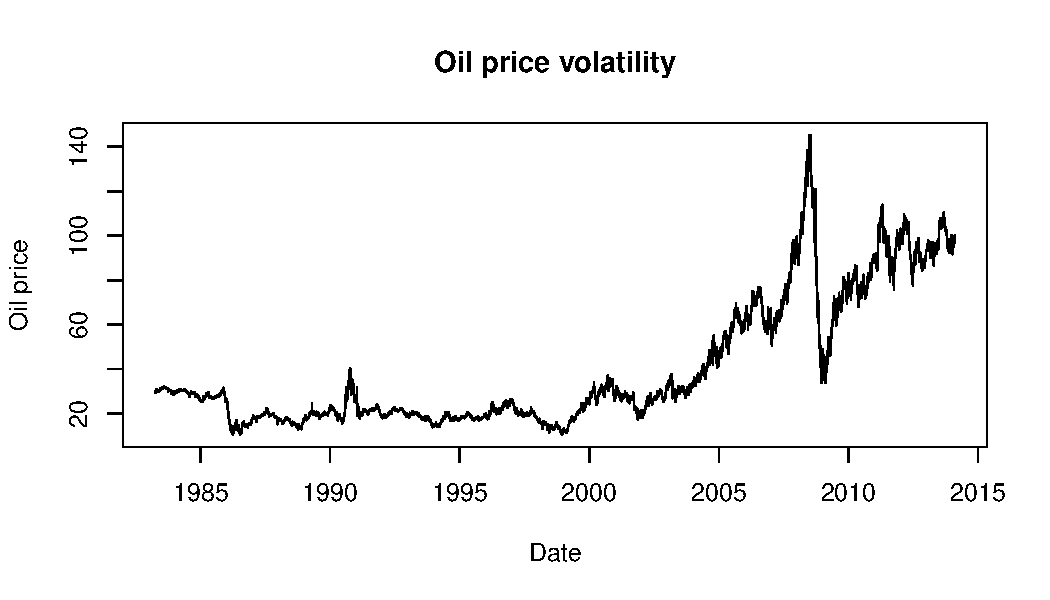
\includegraphics[width=\maxwidth]{figure/oil} \caption[Oil price volatility]{Oil price volatility\label{fig:oil}}
\end{figure}


\end{knitrout}

Figure \ref{fig:oil} shows the fluctuations in the oil price over the last 30 years.  It is clear that there is a lot of risk in some commodities.  However, the most important issue from the point of fund management is the level of correlation between the returns in these other assets and existing asset classes.  The greater the correlation, the smaller the benefit from investing is someting exotic.  The corerlation between the returns may be something that you investigate in your assignment.   

\section{Asset allocations}
You should complete the asset allocation with figures for the proportion of assets that you will hold in the portfolio.  You should justify the reason for having a particular proportion of your portfolio in a particular asset.  You should speak about diversification and you should consider risk. 


You can use something like the \href{https://www.fidelity.co.uk/investor/funds/find-funds/fund-evaluator/fund-evaluator.page}{Fidelity Fund Evaluator} to take a look at how funds allocate their assets.  


\end{document}
